\documentclass[handout]{beamer}
\usepackage[francais]{babel}
\usepackage[utf8]{inputenc}
\usepackage[T1]{fontenc}
\usepackage{graphicx}

\setbeamerfont{page number in head/foot}{}
\setbeamertemplate{footline}[frame number]
\setbeamertemplate{blocks}[shadow=false]

\definecolor{blue1}{rgb}{0.20,0.20,0.70}
\setbeamercolor{block title}{fg=white,bg=blue1}
\setbeamercolor{block body}{fg=black,bg=blue1!10}


\title{Projet de microprocesseur}
\author{Nicolas J., Elie M., Aurélien D. et Louis G.}
\date{28 janvier 2014}

\begin{document}

\begin{frame}
  \maketitle
\end{frame}

\section*{Introduction}

\begin{frame}{Vue d'ensemble}
  \begin{figure}
    \centering
    \includegraphics[width=\textwidth,height=0.9\textheight,keepaspectratio]{organisation}
  \end{figure}
\end{frame}

\begin{frame}{Sommaire}
  \tableofcontents
\end{frame}


\section{Simulateur} % Nicolas et Élie

\begin{frame}{Simulateur - Fonctionnement général}
  \begin{itemize}
  \item Parseur de netlist
  \item Optimizer (ordonne et simplifie les netlists)
  \item Parseur de fichier de ROM
  \item Lecture/Écriture des entrées/sorties du circuit
  \item Initialisation
  \item Cœur du simulateur
  \end{itemize}
\end{frame}
% Décomposé en Optimisation | Utilisation (ROM & entrées/sorties)

\begin{frame}{Simulateur - Fonctionnement interne}
  
  \begin{block}{Optimizer}
    \begin{itemize}
    \item Successeur du Scheduler
    \item Suppression des nappes (sauf vers RAM et ROM)
    \item Suppression des doublons
    \item Problèmes de complexité
    \end{itemize}
  \end{block}
  
  \pause
  
  \begin{block}{Simulation}
    \begin{itemize}
    \item Problèmes d'optimisation
    \item Phase d'initialisation pour modifier la structure des données
    \end{itemize}
  \end{block}
  
\end{frame}

\begin{frame}{Simulateur - Utilisation}

  \begin{block}{ROM}
    \begin{itemize}
    \item Contient le programme à exécuter.
    \item Décrit par un fichier .bin, suite de 0 et 1 pouvant contenir des commentaires.
    \end{itemize}
  \end{block}
	
  \pause
	
  \begin{block}{Entrées/Sorties}
    \begin{itemize}
    \item Utilisations de l'entrée/sortie standard
    \item Communication avec les périphériques par pipe
    \item Possibilité d'asynchronisation de l'entrée
    \end{itemize}
  \end{block}

\end{frame}



\section{Microprocesseur}
% Nicolas et Élie
\begin{frame}{Microprocesseur - Architecture}
	\begin{figure}
		\centering
		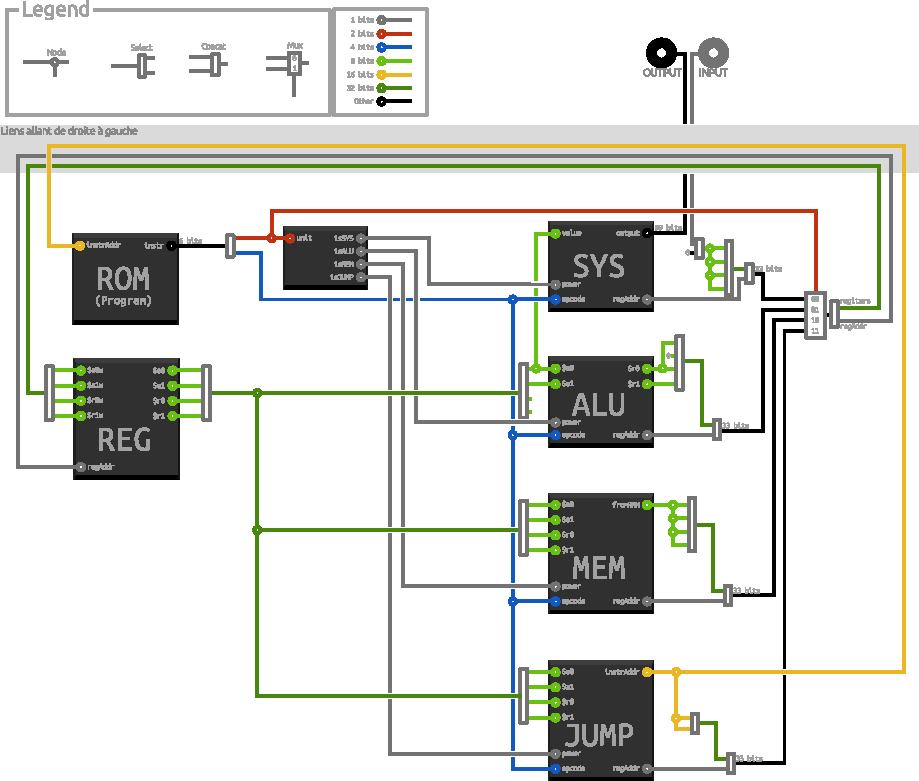
\includegraphics[width=\textwidth,height=0.9\textheight,keepaspectratio]{archi}
	\end{figure}
\end{frame}

\begin{frame}{Microprocesseur - Modification}
	\begin{figure}
		\centering
		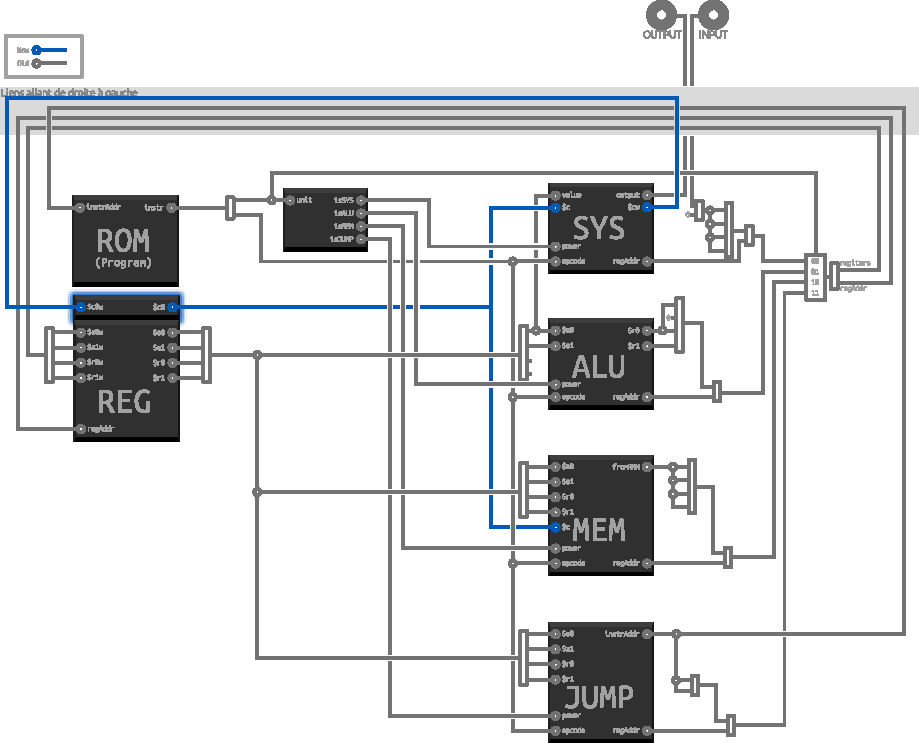
\includegraphics[width=\textwidth,height=0.9\textheight,keepaspectratio]{archi_update}
	\end{figure}
\end{frame}

\begin{frame}{Microprocesseur - Séparation CPU/GPU}
	\begin{figure}
		\centering
		\includegraphics[width=\textwidth,height=0.9\textheight,keepaspectratio]{cpu_gpu}
	\end{figure}
\end{frame}



\section{Programme}
% Louis (TODO)
\begin{frame}{Programme}
	
\end{frame}

\begin{frame}{Programme - Gestion de la mémoire}
	$\overline{\underbrace{\underline{|13|24|29|30|31|32|60|100|}}_{chunk 0}\underbrace{\underline{|j|m|a1|a2|h|mn|s|*|}}_{chunk 1}\underbrace{\underline{|L0|*|L2|*|*|*|*|old|}}_{chunk 2}}$
\end{frame}

\begin{frame}{Programme - Difficultés}
	\begin{itemize}
		\item Difficile de coder avec si peu d'instructions, mais intéressant
		\item Surtout lorsqu'il a fallu prendre en compte le nombre de jours par mois
		\item LUT dans la RAM à l'initialisation
		\item Réinitialisation de la LUT au changement d'années (pour traiter les années bisextiles)
	\end{itemize}
\end{frame}


\section{Afficheurs}
% Aurélien (TODO)
\begin{frame}{Afficheurs}
	
\end{frame}


\section{Oscillateur}
% Élie
\begin{frame}{Oscillateur}
	\begin{figure}
		\centering
		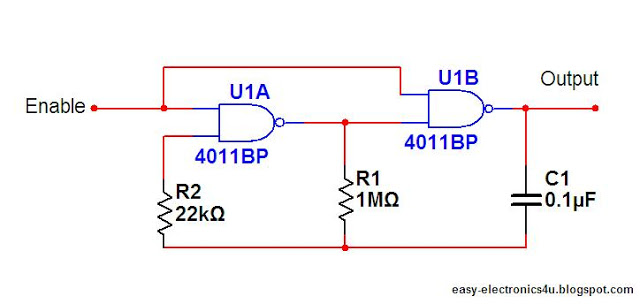
\includegraphics[width=\textwidth,height=0.9\textheight,keepaspectratio]{oscillator.jpg}
	\end{figure}
\end{frame}

\begin{frame}{Oscillateur - Montage}
	\begin{figure}
		\centering
		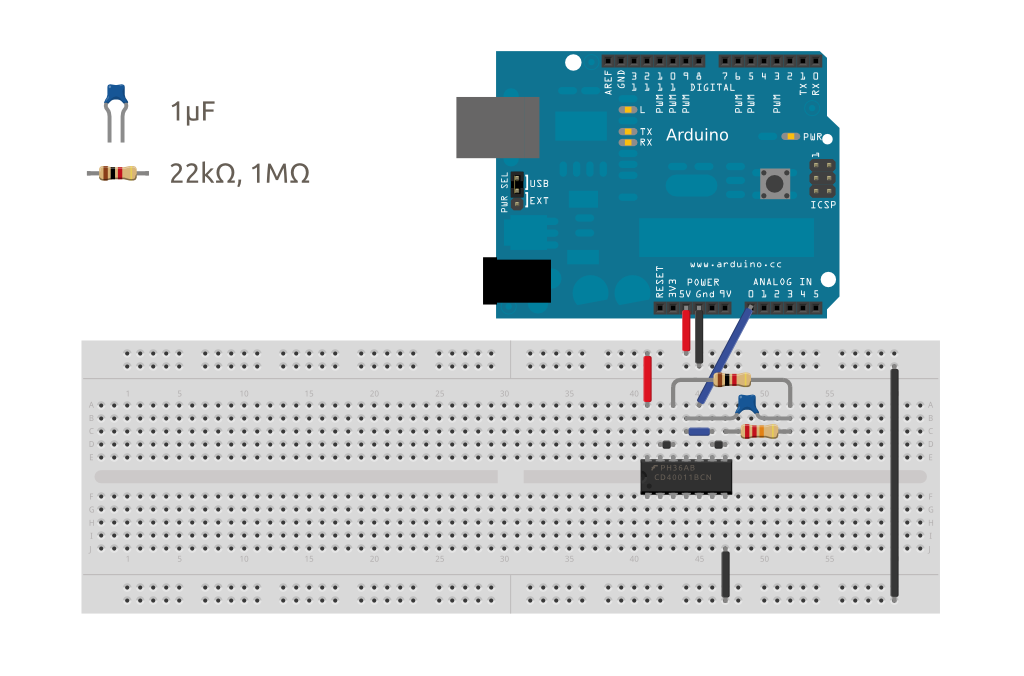
\includegraphics[width=\textwidth,height=0.9\textheight,keepaspectratio]{sysdig_clock}
	\end{figure}
\end{frame}

\begin{frame}{Oscillateur - Mesures pratiques}
\begin{columns}
\begin{column}{0.5\textwidth}
	\begin{figure}
		\centering
		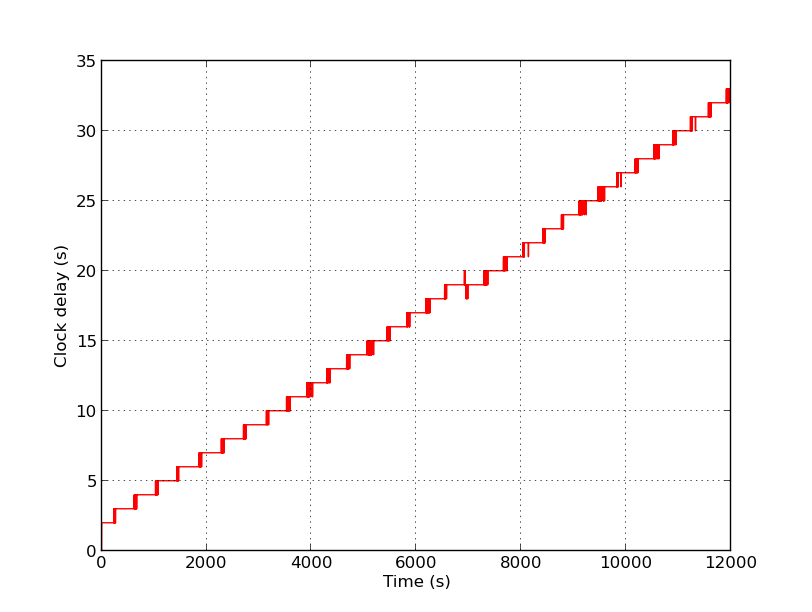
\includegraphics[width=\textwidth,height=0.9\textheight,keepaspectratio]{scale4_int.png}
	\end{figure}
\end{column}
\begin{column}{0.5\textwidth}
	\begin{figure}
		\centering
		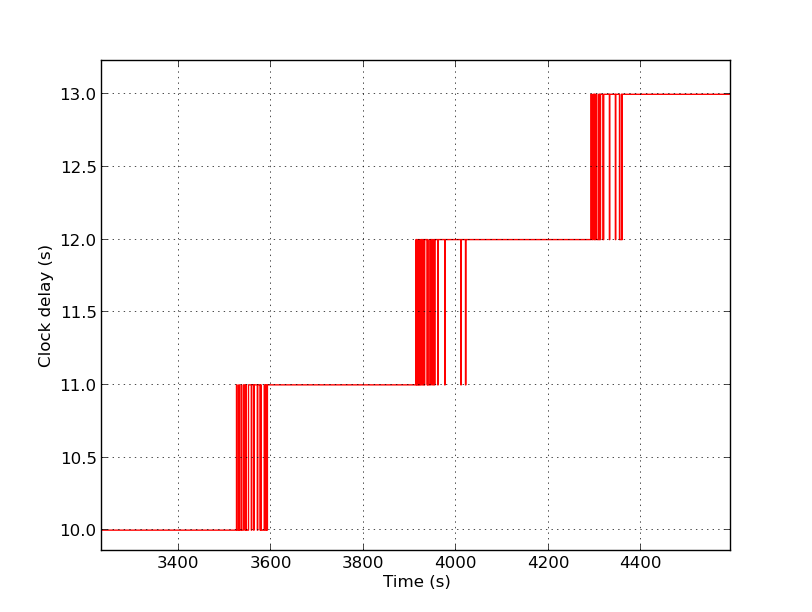
\includegraphics[width=\textwidth,height=0.9\textheight,keepaspectratio]{scale2_int.png}
	\end{figure}
\end{column}
\end{columns}
\end{frame}


\end{document}

